\section{Str\"{o}mungslehre}
Da ein Ziel der Arbeit ist, einen konstanten Strom von Partikeln durch ein bestimmtes Medium zu generieren um letztendlich ein Partikeltestsignal zu bekommen, ist es wichtig grundlegende physikalische Eigenschaften von Str\"{o}mungen zu kennen. Deshalb ist es unumg\"{a}nglich sich im Vorfeld mit den Grundlagen der Str\"{o}mungslehre auseinanderzusetzen.
\\\\
Die Str\"{o}mungslehre ist die Wissenschaft vom physikalischen Verhalten von Fluiden und Gasen. Die in dieser Lehre gewonnenen Kenntnisse sind Gesetzm\"{a}{\ss}igkeiten in Str\"{o}mungsvorg\"{a}ngen und dienen der L\"{o}sung von Str\"{o}mungsproblemen. Dabei liegt der Fokus auf den Problemen bei umstr\"{o}mten oder durchstr\"{o}mten Bauteilen. Gegenstand der Str\"{o}mungslehre sind die Bewegungen von Fluiden, Gasen und ruhenden, flie{\ss}enden oder str\"{o}menden Substanzen. Die Str\"{o}mungslehre l\"{a}sst sich in verschiedene Teilgebiete unterteilen von denen allerdings f\"{u}r diese Arbeit nur die Fluiddynamik relevant ist und die Auslegungen sich daher auf dieses Teilgebiet beschr\"{a}nken werden\cite{stream}.

\subsection{Str\"{o}mungseigenschaften}
Grob betrachtet gibt es zwei wichtige Eigenschaften von Str\"{o}mungen, die f\"{u}r diese Arbeit wichtig sind. Auf der einen Seite gibt es die laminaren Str\"{o}mungen, die man sich als ein gleichm\"{a}{\ss}iges Flie{\ss}en vorstellen kann, auf der anderen Seite als Gegensatz die turbulenten Str\"{o}mungen.
\\\\
In der Fluiddynamik ist die laminare Str\"{o}mung eine Bewegung des Fluids ohne sichtbare Turbulenzen. Dabei str\"{o}mt das Fluid in Schichten, die sich nicht miteinander vermischen. Verwirbelungen treten erst mit h\"{o}heren Str\"{o}mungsgeschwindigkeiten auf, ab diesem Zeitpunkt ist die Str\"{o}mung turbulent.
\begin{figure}[H]
        \myfloatalign
        {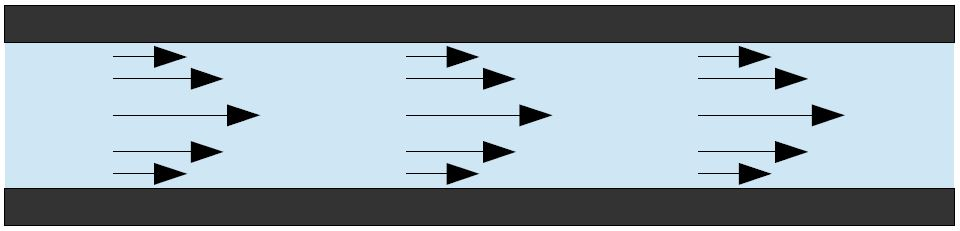
\includegraphics[width=.9\linewidth]{gfx/fundamentals/laminar.jpg}} \quad
        \caption[Laminare Str\"{o}mung]
        {Laminare Str\"{o}mung}
        \label{fig:laminar}
\end{figure}
Im Vergleich dazu ist die turbulente Str\"{o}mung die Bewegung von Fluiden, bei der Verwirbelungen auftreten. Diese Str\"{o}mungsform ist gekennzeichnet durch eine scheinbar zuf\"{a}llig variierende Komponente. Turbulenzen f\"{u}hren zu einer verst\"{a}rkten Durchmischung des Fluids mit der Umgebungsluft. Dabei hat die turbulente Str\"{o}mung eine ungeordnete und schwer vorhersagbare Struktur
\begin{figure}[H]
        \myfloatalign
        {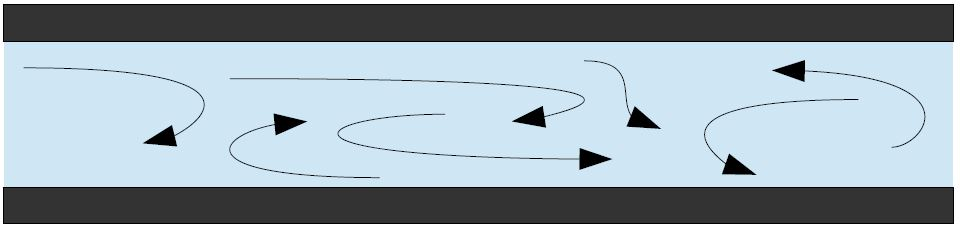
\includegraphics[width=.9\linewidth]{gfx/fundamentals/turbulent.jpg}} \quad
        \caption[Turbulente Str\"{o}mung]
        {Turbulente Str\"{o}mung}
        \label{fig:turbulent}
\end{figure}
F\"{u}r diese Arbeit wurden verschiedene Ideen mit verschiedenen Anforderungen an die Str\"{o}mung entwickelt. Gemeinsam haben alle Konzepte, dass ein laminarer Strom des Fluids am Eingang des Messger\"{a}tes verlangt war. Bei einigen kam noch hinzu, dass das Fluid vor dem Einstr\"{o}men in das Messger\"{a}t mit Luft vermischt werden sollte. Dort will man also eine gezielte turbulente Str\"{o}mung zur Vermischung generieren, die im sp\"{a}teren Aufbau allerdings wieder eine laminare Form annehmen sollte\cite{stream}.
\subsection{Reynolds- und Prandtlzahl}
Die Reynoldszahl ist eine dimensionslose Kennzahl. Sie wird in der Str\"{o}mungslehre als Beurteilungskriterium f\"{u}r laminare Str\"{o}mungen verwendet und ist deshalb relevant f\"{u}r diese Arbeit. Die Reynoldszahl ist definiert durch:
\begin{align*}
{Re} = \frac{\rho vd}{\eta} = \frac{vd}{\nu}
\end{align*}
Dabei ist \(\rho\) die Dichte des Fluids, \(v\) die Str\"{o}mungsgeschwindigkeit des Fluids gegen\"{u}ber dem durchstr\"{o}mten K\"{o}rper und \(d\) die L\"{a}nge des K\"{o}rpers. Die kinematisch Viskosit\"{a}t \(\nu\) des Fluids unterscheidet sich von der dynamischen Viskosit\"{a}t \(\eta = \nu \rho\) durch den Faktor \(\rho\). \"{U}berschreitet die Reynoldszahl einen kritischen Wert \({Re}_{krit}\), wird eine bis dahin laminare Str\"{o}mung anf\"{a}llig gegen kleinste St\"{o}rungen und aus der laminaren Str\"{o}mung wird eine turbulente Str\"{o}mung. In Bezug auf die Arbeit war es also wichtig eine Reynoldszahl zu erreichen, die dem verlangten Str\"{o}mungsbild gen\"{u}gt\cite{reynolds}.
\\\\
Die Prandtl-Zahl ist ebenfalls eine Kennzahl f\"{u}r Fluide und ist ebenfalls dimensionslos. Definiert ist die Prandtl-Zahl als Verh\"{a}ltnis zwischen kinematischer Viskosit\"{a}t und Temperaturleitf\"{a}higkeit:
\begin{align*}
{Pr} = \frac{\nu}{a} = \frac{\eta c_p}{\lambda}
\end{align*}
Hier ist \(a\) die Temperaturleitf\"{a}higkeit des Fluids, \(\nu\) die kinematische Viskosit\"{a}t, \(\eta\) die dynamische Viskosit\"{a}t, \(c_p\) die spezifische W\"{a}rmekapazit\"{a}t und \(\lambda\) die W\"{a}rmeleitf\"{a}higkeit des Fluids. Die Prandt-Zahl stellt eine Verkn\"{u}pfung der Geschwindigkeit mit der Temperatur eines Stoffes dar. Wichtig ist die Prandtl-Zahl, da sie ein Kriterium f\"{u}r die Diffusion von Stoffen ist, also f\"{u}r eine wom\"{o}gliche Vermischung durch Verwirbelungen\cite{prandtl}.